\chapter{Extending \rapidminer}
\label{sec:extending_rapidminer}

The core \rapidminer operators provide solutions for a large amount of usual
data mining applications. However, it is quite simple to write your own 
operators in order to extend \rapidminer. The platform provides the data management,
the nesting of operators, and the handling of optional and mandatory
parameters.

This chapter describes how to implement your own \rapidminer
operator\index{Operator} in Java. At least you should know the basic
concepts of this language to understand what we are doing here. All
necessary information about the \rapidminer classes can be found in the \rapidminer
API documentation which should be available on the \rapidminer homepage \rapidminerurl.


\section{Project structure}
In order to compile your own operators against \rapidminer, you must add
the file \filename{rapidminer.jar} and eventually some other \filename{jar} files in the
\filename{lib} directory of \rapidminer to your \commandline{CLASSPATH}. If
you downloaded the source version of \rapidminer, you should add the
\filename{build} directory (instead of \filename{rapidminer.jar}) to the
\commandline{CLASSPATH}. 

Using the source version of \rapidminer has the advantage that you can use
the \commandline{ant} buildfile. \commandline{ant} is a make-like
open source build tool for Java you can download from
\url{http://ant.apache.org}. The buildfile defines several useful
targets, among which is \commandline{build} which, as one may
easily guess, compiles all sources.

An Emacs JDE project file is also part of the source distribution. JDE
is the Java Development Environment for Emacs and turns Emacs into a
Java IDE. It can be downloaded from
\url{http://jdee.sunsite.dk}. On Unix platforms, Emacs is a widespread
editor but it also runs on Windows. It can be downloaded from
\url{http://www.gnu.org/software/emacs}.

There are also project files for Eclipse in the project folders. Eclipse is a 
powerful open-source IDE for Java which can be downloaded at \url{http://www.eclipse.org}.
It is also very easy to integrate the latest CVS version into Eclipse which is
described in detail at our web page\footnote{\rapidminerurl}.



\section{Operator skeleton}

The first step to do when implementing a new operator is to decide which class
must be extended. If your operator simply performs some action on its input and
delivers some output it should extend the class
\begin{center}
\java{com.rapidminer.operator.Operator}.
\end{center} 
If the operator shall be able to contain inner operators, it must
inherit from
\begin{center}
\java{com.rapidminer.operator.OperatorChain},
\end{center}
which itself extends \java{Operator}. Please refer to the API
documentation if there is a more specific subclass of
\java{Operator} which may serve your purpose. If your operator shall be a
learning scheme it might be useful to implement
\begin{center}
\java{com.rapidminer.operator.learner.Learner}
\end{center}
or extend
\begin{center}
\java{com.rapidminer.operator.learner.AbstractLearner}
\end{center}
though it does not need to. Similar interfaces and abstract operator classes
exists for other purposes too.

Now, there are some important things to specify about your operator.
These specifications will automatically be used for sanity checks, parameter
value checks, creation of GUI elements, and documentation. The following
methods must or should be overridden (if the operator does not inherit from
\java{Operator} directly, this may not be necessary):
\begin{enumerate}
\item One argument constructor: this constructor gets an object of the class 
  \java{OperatorDescription} which must be passed to the superclass by
  invoking \java{super(description)}.
\item \java{Class[] getInputClasses()}: Specifies the number and type of
  objects that are expected as input classes. Only classes that implement
  \java{com.rapidminer.operator.IOObject} may be passed between
  operators. Typical objects passed between operators include example sets,
  models, and performance vectors (see section \ref{sec:op:inandout}).
\item \java{Class[] getOutputClasses()}: Specifies the number and type of
  objects that are generated by this operator as output classes.
\item \java{List<ParameterType> getParameterTypes()}: Specifies the names and types
  of parameters that may be queried by this operator. Please make sure
  to add the parameter types to a \java{java.util.List} retrieved by a
  call to \java{super.get\-Pa\-ra\-me\-ter\-Types()}. The usage of subclasses of
  \java{ParameterType} for this purpose is described in
  sections~\ref{sec:op:adding_parameters} and the retrieval of
  parameter values is described in section~\ref{sec:op:getting_parameters}.
\item \java{IOObject[] apply()}: This is the main method that is
  invoked whenever the operator should perform its work. This method
  can query parameter values, input objects, and maybe call the
  \java{apply} methods of inner operators (in case of an operator chain). It
  returns an array of \java{IOObject}s as a result.\index{Operator!performing action}
  Please note that this method might throw an exception of type
  \java{OperatorException}.
\end{enumerate}

If your operator extends \java{OperatorChain} is must additionally implement
the following methods:
\begin{enumerate}
\item \java{int getMaxNumberOfInnerOperators()} and
  \java{getMin\-Num\-ber\-Of\-In\-ner\-Ope\-ra\-tors()}: these methods specify
  the maximum and minimum number of inner operators allowed for the operator
  chain. Return 0 and \java{Integer.MAX\_VALUE}, respectively for an unlimited
  number of inner operators.
\item \java{InnerOperatorCondition getInnerOperatorCondition()}: Operator
  chains have to implement this method. The delivered condition is used to
  perform checks if all inner operators can handle their input and deliver the
  necessary output. Several implementations for InnerOperatorCondition are
  available, please refer to the API documentation for details.
\end{enumerate}


Please have a look at the simple operator skeleton\index{Operator!skeleton}
showed in figure \ref{fig:operatorskeleton}. As described above, the operator
skeleton extends the class \java{Operator}.

\javafile{operatorskeleton.jav}{operatorskeleton}{Operator skeleton}{Operator skeleton}

The methods \java{getInputClasses()} and \java{getInputClasses()} do
not declare any input and output objects yet and so does the method
\java{getParameterTypes()}, which simply returns the parameters
declared by its superclass. According to these declarations, the
\java{apply()} method does nothing, but quietly returns an empty
array. The following sections describe, how you can fill these methods
with code.

\textit{Note:} Since version 3.0 of \rapidminer\ each operator must have an
one-argument constructor which must at least pass the given operator
description object to the superclass constructor. Please note that
during operator construction the method getParameterTypes() will be
invoked and must be fully functional, i.\,e. not depending on uninitialized
fields of the operator.

Finally, if your operator is implemented and you want to use it from
\rapidminer, you must declare the new operator class by adding a short entry
to an XML file. This is described in
section~\ref{sec:op:declaring_operators}.




\section{Useful methods for operator design}

Before we discuss an easy example for a self-written operator, the required methods are
described in detail. These methods enable you to declare a parameter, query a
parameter value, adding a \java{Value} which can be plotted by the
\op{PocessLog} operator and handling the in- and output of your operator.



\subsection{Defining parameters}
\label{sec:op:adding_parameters}

As we have seen above, the method \java{getParameterTypes()} can be used to
add parameters to your operator. Each parameter is described by a
\java{ParameterType} object, i.e. an object which contains the name, a small
description, and in case of a numerical parameter the range and default
value of this parameter. A new parameter type has to extend the class
\begin{center}
\java{com.rapidminer.parameter.ParameterType}
\end{center} 
In \rapidminer, for each simple data type a parameter type is
provided, e.g. for boolean values the type \java{ParameterTypeBoolean} or
\java{ParameterTypeInteger} for integers.
Table \ref{tab:op:parametertypes} shows all possible parameter types. Please
refer to the API documentation for details on constructing the different
parameter types.

Since the method \java{getParameterTypes()} returns a list of \java{ParameterType}s, your operator should
first invoke \java{super.getParameterTypes()} and add its parameter types to
the list which is returned by this method. In this way it is ensured that the
parameters of super classes can also be set by the user. Figure
\ref{fig:addingparameter} shows how a new integer parameter is added.

\javafile{addingparameter.jav}{addingparameter}{Adding a parameter}{Adding a parameter}

As you can see you create a new \java{ParameterTypeInteger} and add it to the
list. The first argument of the constructor is the name of the parameter which
will be used in the XML description files or in the GUI parameter
table. The second argument is a short description. This is used as tool tip
text when the mouse pointer stays on the parameter in the GUI for some seconds. For numerical
parameter types a range can be specified. The first number defines the minimum
value of this parameter, the second the maximum value. The last number is the
default value which is used when the user do not change this parameter in the
process setup.

Not every operator needs parameters. This is the reason why the method
\java{getParameterTypes()} is not abstract in Operator. You can simply ommit
the implementation of this method if your operator does not use any
parameters. However, you should notice that the method
\java{getParameterTypes()} is invoked by the super-constructor. You should
therefore not use global variables which are not initialized yet.


\newcolumntype{Y}{>{\small\raggedright\arraybackslash}X}
\newcolumntype{Z}{>{\small\tt\raggedright\arraybackslash}X}
\renewcommand{\tabularxcolumn}[1]{p{#1}}
\begin{table}[htbp]
  \begin{tabularx}{\linewidth}{|Z|Y|}
    \hline
    \textbf{Type}                  & \textbf{Description} \\
    \hline\hline
    ParameterTypeBoolean   & A boolean parameter. The defined value can be queried by
    \java{getParameterAsBoolean(key)}. \\
    \hline
    ParameterTypeCategory  & A category parameter which allows defined
    strings. The index of the chosen string can be queried by
    \java{getParameterAsInt(key)}. \\
    \hline
    ParameterTypeColor     & A parameter for colors. This is currently only
    used for user interface settings. The specified color can be queried by
    \java{getParameterAsColor(key)}. \\
    \hline
    ParameterTypeDirectory & A directory. The path to the chosen directory
    can be queried by \java{getParameterAsString(key)}. \\
    \hline
    ParameterTypeDouble    & A real valued parameter. The defined value can be queried by
    \java{getParameterAsDouble(key)}. \\
    \hline
    ParameterTypeFile      & A file. The path to the chosen file can be queried
    by \java{getParameterAsString(key)}.\\
    \hline
    ParameterTypeInt       & A integer parameter. The defined value can be queried by
    \java{getParameterAsInt(key)}. \\
    \hline
    ParameterTypeList      & A list of parameters of another parameter
    type. The defined list can be queried by \java{getParameterList(key)}. \\
    \hline
    ParameterTypePassword  & A password parameter. Passwords are masked with *
    in the GUI and queried by the system if the user has not specified the password in
    the process setup. The defined string can be queried by \java{getParameterAsString(key)}. \\
    \hline
    ParameterTypeString         & A simple string parameter. The defined value can be queried by
    \java{getParameterAsString(key)}. \\
    \hline
    ParameterTypeStringCategory & A category parameter which allows defined
    strings. Additionally the user can specify another string. The chosen
    string can be queried by \java{getParameterAsString(key)}. \\
    \hline
  \end{tabularx}
  \caption[Parameter types]{These parameter types can be added to your operator. Please refer
    to the API documentation for details on creation.}
  \label{tab:op:parametertypes}
\end{table}



\subsection{Getting parameters}
\label{sec:op:getting_parameters}

Now you can add  different parameter types to your operator. For each type 
\begin{center}
ParameterTypeXXX
\end{center}
a method \java{getParameterAsXXX()} is provided by the superclass
\java{Operator} unless another method is described in table
\ref{tab:op:parametertypes}\index{parameter}. All these methods return
an appropriate Java type, e.g. \java{double} for \java{getParameterAsDouble()}. 
Table~\ref{tab:op:parameters} shows the parameter getter methods of
the class \java{Operator} in detail.

The methods \java{getParameterAsXXX()} will throw an UndefinedParameterError
if the user has not defined a value for a non-optional parameter without
default value. Since this Error extends UserError which extends
OperatorException you should just throw these error out of your apply
method. A proper GUI message will be automatically created.

The List returned by \java{getParameterList(String)} contains
Object arrays of length 2. The first object is a key (String) and the second
the parameter value object, e.g. a Double for ParameterTypeDouble.


\newcolumntype{Y}{>{\small\raggedright\arraybackslash}X}
\newcolumntype{Z}{>{\small\tt\raggedright\arraybackslash}X}
\renewcommand{\tabularxcolumn}[1]{p{#1}}
\begin{table}[htbp]
  \begin{tabularx}{\linewidth}{|Z|Y|}
    \hline
    \textbf{Method}                  & \textbf{Description} \\
    \hline\hline
    getParameterAsBoolean(String key) & Returns a parameter and
    casts it to boolean.\\
    \hline
    getParameterAsColor(String key)   & Returns a parameter and
    casts it to Java Color.\\
    \hline
    getParameterAsDouble(String key)  & Returns a parameter and
    casts it to double. \\
    \hline
    getParameterAsFile(String key)    & Returns a parameter and
    casts it to a Java File.\\
    \hline
    getParameterAsInt(String key)   & Returns a parameter and
    casts it to int.\\
    \hline
    getParameterAsString(String key) & Returns a parameter and
    casts it to String.\\
    \hline
    getParameterList(String key) & Returns a parameter and casts
    it to a Java List. \\
    \hline
  \end{tabularx}
  \caption{Methods for obtaining parameters from {\tt Operator}}
  \label{tab:op:parameters}
\end{table}



\subsection{Providing \java{Value}s for logging}
\index{values!providing}

As you can see, the operator skeleton contains a one-argument
constructor which must pass the given description object to the
super-constructor. This is necessary for the automatic operator
creation with help of factory methods (see section
\ref{sec:integrating_rapidminer}). These constructors can also be used to declare
\java{Value}s which can be queried by an \op{ProcessLog} operator
(see \ref{sec:op:ProcessLog}). Each value you want to add must extend 
\begin{center}
\java{com.rapidminer.operator.Value}
\end{center}
and override the abstract method \java{getValue()}.
Figure \ref{fig:addvalues} shows how you can add some values in the constructor of
your operator. Note that usually non-static inner classes are used to
extend \java{Value}. These classes have access to private fields of
the operator and may, e.g. return the number of the current run, the
current performance or similar values.

\javafile{addvalues.jav}{addvalues}{Adding \java{Value}s to your Operator which
  can be queried by \op{ProcessLog}.}{Adding \java{Value}s to your Operator}

\emph{Note:} Please make sure that the only purpose of an operator's
constructor should be to add values and \emph{not} querying parameters or
perform other actions. Since the operator description and parameters will be
initialized after operator construction these type of actions will probably
not work and might cause exceptions.




\subsection{Input and output}
\label{sec:op:inandout}

As default, operators consume their input by using it. This is often a
useful behavior, especially in complex process definitions. 
For example, a learning operator consumes an example set to produce a
model and so does a cross validation to produce a performance value of
the learning method. To receive the input \java{IOObject} of a certain
class simply use
\begin{center}
\java{<T extends IOObject> T getInput(Class<T> class)}
\end{center}
This method delivers the first object of the desired class which is in the
input of this operator. By using generics it is already ensured that the
delivered object has the correct type and no cast is necessary. 
The delivered object is consumed afterwards
and thus is removed from input. If the operator alters this object, it
should return the altered object as output again. Therefore, you have
to add the object to the output array which is delivered by the
\java{apply()} method of the operator. You also have to declare it in
\java{getOutputClasses()}.
All input objects which are not used by your operator will be
automatically passed to the next operators. 

\emph{Note:} In versions before 3.4 it was necessary to cast the delivered
object to the correct type. This cast is no longer necessary.

In some cases it would be useful if the user can define if the input
object should be consumed or not. For example, a validation chain like
cross validation should estimate the performance but should also be
able to return the example set which is then used to learn the overall
model.
Operators can change the default behavior for input consumation and
a parameter will be automatically defined and queried. The default
behavior is defined in the method \java{getInputDescription(Class cls)} 
of operator and should be overriden in these cases. Please
note that input objects with a changed input description must not be
defined in \java{getOutputClasses()} and must not be returned at the
end of apply. Both is automatically done with respect to the value of
the automatically created parameter. Figure \ref{fig:inputdescription}
shows how this could be done. Please refer to the Javadoc comments of
this method for further explanations.

\javafile{inputdescription.jav}{inputdescription}{Changing the input handling behavior of your operator. In this case, example sets should be consumed per default but a parameter named \java{keep\_example\_set} will be automatically defined.}{Changing the input handling behavior of your operator}




\subsection{Generic Operators}
\label{sec:op:generic}

Sometimes a generic operator class should be implemented which should provide
more than one operator. In this case several operators can be declared to
\rapidminer (see section \ref{sec:op:declaring_operators}) with the same class but
different names. The subtype or name of an operator can be requested by
\java{getOperatorClassName()} which is a method of operator. Although this is very
similar to define the operator type with help of a parameter, subtypes can be
used in more subtile way: they can already be used to define the parameters and
therefore each subtype of an operator class may have other parameters. This
feature is used to provide a normal \rapidminer operator with different parameter
types for each Weka operator with the help of only one (short)
class. Please check the source code of the Weka learners for an example of a
generic operator.



\section{Example: Implementation of a simple operator}

After these technical preliminary remarks we set an example
which performs a very elementary task: It should write all examples of
an \ioobj{ExampleSet} into a file. First we consider that all we need as
input for this operator is an example set. Since we will not
manipulate it, we deliver the same example set as output. Therefore the methods
\java{getInputClasses()} and \java{get\-Out\-put\-Cla\-sses()} will only contain
one class: \java{com.rapidminer.example.ExampleSet}. If \ioobj{ExampleSet} is
not contained in the output of the former operator, your operator can not work
and \rapidminer\ will terminate at the beginning of the process. 

Your operator uses one parameter: A file where it should store the
examples. Therefore a \java{ParameterTypeFile} is added to the parameter
list. The third argument in the constructor indicates that this parameter is
mandatory.
Let us presume that your own operators are in the package
\java{my.new.operators}. Please have a look at the operator in figure
\ref{fig:examplesetwriter}, then we will explain the apply() function in detail.

\javafile{examplesetwriter.jav}{examplesetwriter}{Implementation of an
  example set writer}{Implementation of an example set writer}

The first line in \java{apply()} fetches the name of the file to
write the example set to. This method returns the value of the
parameter ``example\_set\_file'', if it is declared in the operator section
of the process configuration file. Since this parameter is mandatory
the process ends immediately with an error message if this parameter is not given.

We need the input example set to iterate through the examples and write them
to a file. We simply use the \java{getInput(ExampleSet.class)} method in order 
to get the desired input object (the example set). 

\emph{Note:} Please note that a cast to \java{ExampleSet} is not necessary. 
For \rapidminer versions before 3.4 a cast to the actual type has to be performed.

Then a stream to the specified file is opened
and an iterator over the examples is created. With this
\java{Iterator<Example>} you can pass through the examples of an example set
like the way you do with a \java{List} iterator. For each example the
values are written into the file and afterwards the stream to the file
is closed. Each operator can throw an \java{OperatorException} to the
calling operator, which would be done if any exception occurred during
writing the file. In this case the thrown exception is an \java{UserError}
which is used because writing presumably fails because the file is not
writable. We will discuss the error handling in section
\ref{sec:op:logservice}.

\emph{Note:} In versions before 3.4 the iterator was called \java{ExampleReader}.
Changing to the generic \java{Iterator<Example>} also allows for the nice new
for-loop introduced in Java 5.0: \java{for (Example e : exampleSet) \ldots}.

The last thing to do is creating a new array of 
{\tt IOObjects} which contains only the used \ioobj{ExampleSet} since no
additional output was produced.
The next section describes the iterating through an example set in detail,
then the exception concept will be explained.



\subsection{Iterating over an \ioobj{ExampleSet}}

\rapidminer\ is about data mining and one of the most frequent applications
of data mining operators is to iterate over a set of examples. This
can be done for preprocessing purposes, for learning, for applying a
model to predict labels of examples, and for many other tasks. We have seen
the mechanism in our example above and we will describe it below.

The way you iterate over an example set is very similar to the concept
of iterators, e.g. in terms of \java{Lists}. The methods which are provided
have the same signature as the methods of a Java \java{Iterator}. The first
thing you have to do is to create such an iterator. The following code 
snippet will show you how:

\javafile{examplereader.jav}{examplereader}{Creating and using an example
  iterator}{Creating and using an example iterator}

Assume \java{exampleSet} is a set of examples which we get from the input
of the operator. First of all, an iterator is created and then we traverse
through the examples in a loop. These iterators are backed up by different
implementations of the interface \java{ExampleReader}. The
classes \ioobj{ExampleSet}\index{ExampleSet},
\ioobj{ExampleReader}\index{ExampleReader}, and
\ioobj{Example}\index{Example} are provided within the package
\java{com.rapidminer.example}. Please check the \rapidminer\ API documentation to
see what else can be done with example sets and examples.



\subsection{Log messages and throw Exceptions}
\label{sec:op:logservice}

If you write your operator, you should make some logging messages
so\index{messages}\index{logging} that users can understand what your
operator is currently doing. It is especially reasonable to log error messages as
soon as possible. \rapidminer\ provides some methods to log the messages of
an operator. We distinguish between {\em log messages} and {\em
results}\index{results}. Of course you can write your results into the
normal log file specified in the process configuration file. But
the intended way to announce results of the process is to use a
\op{ResultWriter} (see section
\ref{sec:op:ResultWriter})\index{ResultWriter@{\op{ResultWriter\/}}} which writes each
currently available result residing in his input. For this purpose two classes
exist, a class \java{LogService} and a class
\java{ResultService}\index{LogService}\index{ResultService}. The latter
can be used by invoking the static method 
\begin{center}
\java{logResult(String result)}
\end{center}
or by simply using a \op{ResultWriter} as described above.

The class \java{com.rapidminer.tools.LogService} provides the static method 
\begin{center}
  \java{logMessage(String message, int verbosityLevel)}
\end{center}
to log text messages. Possible verbosity levels are \java{MINIMUM}, \java{IO},
\java{STATUS}, \java{INIT}, \java{WARNING}, \java{EXCEPTION}, \java{ERROR}, \java{FATAL}, and
\java{MAXIMUM} which are all public constant static fields of
\java{LogService}. The verbosity levels \java{IO} and \java{INIT} should \emph{not}
be used by operator developers. Normal log messages should be logged with
verbosity level \java{STATUS}.


\subsection{Operator exceptions and user errors}

The best way to abort the process because of an error is throwing an
\java{OperatorException}. If the error occurred due to an unforseen
situation, an instance of \java{OperatorException} should be
thrown. To ease bug tracking, it is useful to pass RuntimeExceptions
to the OperatorException constructor as the \java{cause} parameter.
If the error was caused by wrong usage of the operator, e.g. missing
files, or wrong parameter values, an instance of \java{UserError}
should be thrown. An error code referencing an error message in the
file \filename{resources/UserErrorMessages.properties} must be passed
to the constructor of a \java{UserError}. These messages are formatted
using an instance of \java{MessageFormat}. Index numbers in curly
braces are replaced by the arguments passed to the \java{UserError}
constructor. Please refer to the API documentation for construction
details.




\section{Building operator chains}

Now you can extend \rapidminer\ by writing operators which perform tasks on a
given input and deliver the input or additional output to a
surrounding operator. We have discussed the specifications to create
the operator in such a way that it can be nested into other
operators. But what we have not seen is the possibility to write your
own operator chain, i.e. operators which contain inner operators to
which input will be given and whose output is used by your
operator. What transmutes a simple operator to an operator chain is the
possibility to contain other inner operators.

The way you create an operator chain is straightforward: First your
operator does not directly extend \java{Operator} any longer, 
but \java{OperatorChain}\index{OperatorChain@{\op{OperatorChain\/}}}
instead. Since \java{OperatorChain} extends \java{Operator} itself you still have to
implement the methods discussed above. 


The second thing you have to do is to declare how many inner operators
your operator can cope with. Therefore every operator chain has to
overwrite two abstract methods from \java{OperatorChain}:
\index{Operator!inner}
\begin{center}
\java{int getMinNumberOfInnerOperators()}
\end{center}
and
\begin{center}
\java{int getMaxNumberOfInnerOperators()}
\end{center}
which returns the minimum and maximum number of inner operators. If
these numbers are equal, your operator chain must include exactly this number
of inner operators or \rapidminer\ will terminate at the beginning of an
process. 


There is another method which you have to implement:
\begin{center}
\java{InnerOperatorCondition getInnerOperatorCondition()}
\end{center}
This method delivers a condition about the inner operators. This condition should
ensure that the current process setup is appropriate and all inner
operators can be executed. Several implementations of
\java{InnerOperatorCondition} are available, please check the API for further
details. We will explain both methods in detail when we discuss the example in
section \ref{sec:operatorchainexample}.



\subsection{Using inner operators}

You can simply use inner operators via the method 
\begin{center}
\java{getOperator(int index)}
\end{center}
which delivers the inner operator with the given index. You can invoke the
\java{apply()} method of this operator yourself. The \java{apply()} method of the
superclass automatically performs the actions of the inner operators. \rapidminer\
takes care of the sequential execution.



\subsection{Additional input}
\label{sec:io_container}
But what if you want to add additional {\tt IOObjects} to the input of an
inner operator? A cross-validation operator for example, divides an
example set into subsets and adds certain subsets to the input of a
learning operator and others to the input of an operator chain which
includes a model applier and a performance evaluator. In this case your
operator has to consume the original {\tt IOObject} and add others to the
input of the inner operators.\index{Operator!input}

In section \ref{sec:op:inandout} we have seen how an operator can get
the input. This is consumed per default. If your operator should add a
certain {\tt IOObject} to the input of an inner operator it simply has
to call the \java{apply()} method of the inner operator in a way like
\begin{center}
\java{apply(getInput().append(new IOObject[] \{ additionalIO \}))}
\end{center}
or
\begin{center}
\java{apply(new InputContainer(new IOObject[] \{ additionalIO \}))}.
\end{center}
The method \java{getInput()} delivers the \rapidminer container which
provides the input and output objects of the
operators\footnote{\java{com.rapidminer.operator.IOContainer}}\index{IOContainer}.
You can add an array of additional {\tt IOObjects} using the \java{append()}
method. The latter variant ignores the input for the current operator
chain and produces a new input container for the child operators.

You should also use this method if you want to use the same {\tt IOObject} as
input for an inner operator several times, e.g. in a loop, or if you
want to add more than one {\tt IOObject} to the input of an inner operator.



\subsection{Using output}

Inner operators can produce output which your surrounding operator
must handle. The call of the \java{apply(IOContainer)} method of an inner
operator delivers a container like the one described above. You can
get the {\tt IOObjects} out of this container with some
\java{getter}-methods provided by this class. Figure
\ref{fig:innerop} shows the methods to append additional input for
the inner operator and getting specified output from the result of the
\java{apply()} method. The example set is split before into training and test
set\index{Operator!output}.

\javafile{innerop.jav}{innerop}{In- and output of an inner operator}{In- and output of an inner operator}

Mostly you do not need to do anything about adding additional input or
getting the output and \rapidminer\ will manage the in- and output for your
operator. Pay attention to the fact that you do not need to care about the
learned model: \rapidminer\ copes with the learned model for your model applier.




\section{Example 2: Implementation of an operator chain}
\label{sec:operatorchainexample}

The following example does not make much sense for data mining purposes, but
it demonstrates the implementation of an operator chain. Figure
\ref{fig:operatorchainexample} shows the complete code.

\javafile{operatorchainexample.jav}{operatorchainexample}{Example implementation of an operator chain.}{Example implementation of an operator chain.}

All methods inherited of \java{Operator} are implemented as described
above. Since this operator chain uses no parameters, the method
\java{getParameterTypes()} is not overwritten. This operator chain must have
at least one inner operator, the maximum number of inner operators is the
biggest integer which Java can handle. The method which returns the estimated
number of steps of this operator chain makes use of a method of the superclass
\java{OperatorChain}: \java{getNumberOfChildrenSteps()} returns the sum of all
children's steps. 

The purpose of this operator chain is described in the \java{apply()}
method. This operator expects an example set as input and clones it before it
uses the clone as input for each of the inner operators. The inner operators
must produce a performance vector. These vectors are averaged and then
returned.

The desired in- and output behaviours of inner operators must be described
with a condition object returned by the method
\java{getInnerOperatorCondition()}. In this example each inner operator should
be able to handle an example set and deliver a performance vector.






\section{Overview: the data core classes}
\label{sec:data_core}

It will be sufficient for many data mining purposes to iterate through
the example set. However, in some cases one must perform some more
complex changes of data or meta data. \rapidminer tries to hide the
internal data transformations for typical data mining purposes. It
uses a view mechanism to make a trade-off between efficient data
mining data transformations and the usage of memory. In this section
we discuss some basic concepts of the data handling in \rapidminer to
support users who want to write more complex operators.

\begin{figure}[thbp]
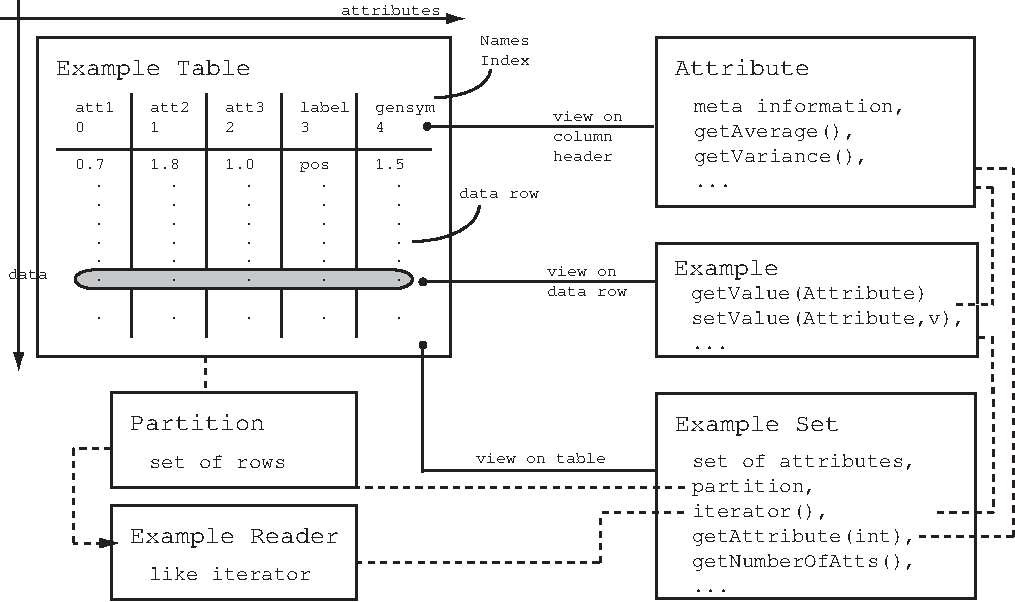
\includegraphics[width=\linewidth]{graphics/data_core.pdf}
\caption[Main classes for data handling]{The main classes used for
  data handling in \rapidminer. The central class is \java{ExampleTable}
  which keeps all data loaded and generated during
  processes. However, it is almost never directly used by operators.}
\label{fig:data_core}
\end{figure}


Figure \ref{fig:data_core} shows the main classes and interfaces which
are used for data handling in \rapidminer. The class \java{ExampleTable}
keeps all data which is loaded or generated during processes and
stores it in one table. The columns are defined by \java{Attribute}s,
which are used for two purposes: managing meta data about table columns
and referring to columns when one asks for the data in one cell. One
might say, that \java{Attribute} is a view on the header of a column
in the data table. Each row of the table is given by a
\java{DataRow}. Although the table is the central class for data
management, \rapidminer developers almost never use it directly. The other
classes shown in Figure \ref{fig:data_core} are used to encapsulate
the functionality and provide more convenient and secure ways to alter your
data.

Since \rapidminer is a data mining environment we often work on data. This
data is, as you know, given as \java{ExampleSet}s. Example sets
consist of a set of attributes and a partition. It is important to
understand, that example sets not keeps the data itself. That means
that you can copy an example set without copying the data. An example
set is merely a view on the example table\footnote{This is the reason
  why the index of an attribute in the example set is not in general
  equal to the index in the example table. To ask for the value of an
  attribute the \java{Attribute} object should always be used instead
  of the index.}.

An important method of example sets is the creation of an example
reader to iterate over the data. Depending whether the example set is
splitted with a partition, a particular instance of an example reader
is returned by the method \java{iterator()}. If only a
partition of examples is used, the returned example reader skips the
deselected examples. Applying weights
for attributes also requires a particular example reader, which
construct examples based on the weights. \rapidminer provides interfaces and
an adaptor concept for example sets to ensure the nestability of the
operators and the used example sets and readers.

The last important class in the data management of \rapidminer is
\java{Example} which is a view on a data row. Examples are constructed
on the fly by the current example reader of the used example set. The
current data row from the example table is used to back up the example
and weights are applied if a weighting or selection should be
applied. Since the indices of attributes in example sets and tables
must not be equal, the query for an attribute's value of an example
should always be performed with help of the attribute and not of it's
index.

Several subclasses exist for example set, example table, and example
reader. These subclasses provide different forms of data management
(main memory, database,\ldots) and views on your data. This concept ensures
data transparency for all operators and the nesting of operators. In
addition, new classes can be easily written to extend \rapidminer for
special purposes.





\section{Declaring your operators to \rapidminer}
\label{sec:op:declaring_operators}
At this point you know all the tricks to write your own operators and
the tool kit which is provided by \rapidminer for this purpose. The last
thing you have to do is to declare your operator to \rapidminer. Every
operator must comply with the following terms\index{Operator!declaring}:

\begin{description}
  \item[name] A meaningful name to specify the operator in a process 
    configuration file is required. The name must be unique.
  \item[class] The fully classified classname of your operator (must be in your
    java {\tt CLASSPATH} variable).
  \item[description] A short description of your operator and its task.
  \item[deprecation] A short description why your operator is deprecated and a short description of a workaround.
  \item[group] A name of a group. This may be your own group or one of the predefined
  \rapidminer group names.
  \item[icon] This is also optional but can be used to ease identification of
  the operator.
\end{description}

The definition of deprecation and icon are optional. If deprecation is omitted,
the operator is simply not regarded as deprecated - which is pretty much the default.
If icon is missing, the default icon for the operator group is used.
To link these description parts to one another you have to specify them in a
operator description file.
Every entry holds for one
operator and they are written like the ones in figure
\ref{fig:operators}. We assume that you save these descriptions in a file
named 'operators.xml'.

\examplefile{operators.xml}{operators}{Declaring operators to \rapidminer}

Additionally to simple operator entries you can specify one or more operator
factory classes which must implement the interface
\begin{center}
\java{com.rapidminer.tools.GenericOperatorFactory}.
\end{center}
This is especially useful if you want to provide more than one operator for
each class by working with operator subtypes. This is the preferred way to add 
generic operators with one class but more than subtype or operator name.

In order to use your operators with \rapidminer\ you have to add them to your {\tt
  CLASSPATH} variable. Then you can start \rapidminer\ with the option 
\begin{center}
\java{-Drapidminer.operators.additional=path/to/your/operators.xml}
\end{center}
Please edit your start scripts and add the parameter to the line which starts
\rapidminer\ or start \rapidminer\ manually with a call like

\java{java} \\
\java{-cp \$RAPIDMINER\_HOME/lib/rapidminer.jar:your/class/path} \\
\java{-Drapidminer.home=\$RAPIDMINER\_HOME} \\
\java{-Drapidminer.operators.additional=path/to/your/operators.xml} \\
\java{com.rapidminer.gui.RapidMinerGUI}

Your new operators should be available now and can be chosen in the GUI. More
than one additional operator description file can be specified by making use
of the system dependent path separator, for unix systems for example with 

\java{-Drapidminer.operators.additional=my\_operators.xml:other\_ops.xml} \\








\section{Packaging plugins}
\index{plugins!authoring}
\label{sec:plugins_packaging}
If you want to make your operators available for download, you can easily
create plugins.
\begin{enumerate}
\item Compile your Java sources.
\item Create a file named \filename{operators.xml} as described above
\item Create a jar archive using the \commandline{jar} command that comes with the
  JDK. The archive must contain your operator class files and all classes they
  depend on. The file \filename{operators.xml} must go into the
  \filename{META-INF} directory of the archive.
\item If desired, create a file named \filename{ABOUT.NFO} and add it
  to the \filename{META-INF} directory of the jar file.
\item IMPORTANT: You have to use a \filename{Manifest} file in the Jar archive.
  In this manifest file the entry \java{RapidMiner-Type} with the value 
  \java{RapidMiner\_Plugin} has to be used in order to make this Jar archive
  to a valid RapidMiner plugin (since version 4.2)! Additionally, the entries
  Implementation-Title, Implementation-Version, Implementation-Vendor,
  Implementation-URL, \rapidminer-Version, and Plugin-Dependencies will be evaluated
  by \rapidminer. \rapidminer-Version defines the minimum \rapidminer version which is needed for
  this plugin. Plugin-Dependencies must have the form \\
  plugin\_name1 [plugin\_version1] \# \ldots \# plugin\_nameM [plugin\_versionM]
\item You can include GUI icons for your operators within the
  jar file. If you set the \tag{icon} attribute of the \tag{<operator>} tag
  in the \filename{operators.xml} file to ``foo'', \rapidminer will look for a
  file named \filename{op\_foo.gif} in the directory
  \filename{com/rapidminer/resources/icons/groups/24} or in the directory 
  \filename{com/rapidminer/resources/icons/operators/24} of the jar file.
\item Copy the archive into \filename{lib/plugins} directory. If you like, also put
  it on your website or send it to us. Since \rapidminer is licensed under the GNU
  General Public License you have to develop your plugins as opensource
  software and you have to make it available for the \rapidminer community. If this
  is not possible for any reasons, e.g. because the development of the plugin
  was done for commercial purposes, you should contact us for a special
  commercial version of \rapidminer.
\end{enumerate}
Hint: If your plugin depends on external libraries, you do not have to
package these into one archive. You can reference the libraries using a
\commandline{Class-Path} entry in your jar \filename{Manifest} file.
For information on installation of plugins, please refer to
section~\ref{sec:plugins_installing}.




\section{Documentation}
The operator reference chapter of the  \LaTeX{} \rapidminer tutorial is
generated using the Javadoc class comments of the operator source
code. Therefore some additional Javadoc tags can be used. 
\begin{description}
\item[@rapidminer.xmlclass] The classname given in the
  \filename{operators.xml} if different from the classname.
\item[@rapidminer.index] For \LaTeX output generate an index entry for the
  tutorial referring to the description of this operator.
\item[@rapidminer.reference] A BibTeX key that will be used to generate a
  HTML bibliography entry. Ignored for \LaTeX{} output.
\item[@rapidminer.cite] Inline tag. For \LaTeX{} output generate a citation. For HTML
  output, simply print the key.
\item[@rapidminer.ref] Inline tag. For \LaTeX{} output generate a reference
  to a tutorial section, for HTML simply print the reference name.
\item[@rapidminer.xmlinput] The text of this tag must consist of three
  strings separated by a pipe symbol ("$|$"). The first string must be
  a filename, the second must be a label, and the third must be a
  caption for a figure. The file specified will be input both in HTML
  and \LaTeX{} documentation.
\end{description}
Please refer to the API documentation of the class
\begin{center}
com.rapidminer.docs.DocumentationGenerator
\end{center}
to learn how the documentation for your operators can automatically created
from your Java source code and Javadoc comments.
 


\section{Non-Operator classes}

Some operators, like \op{PerformanceEvaluator} and the
\op{ExampleFilter}, have parameters that let you specify
implementations of certain interfaces that will solve simple
subtasks, e.g. determining which of two performance vectors is
preferable, or which examples to remove from an example set. Those classes
must be specified with the fully qualified classname. If you want to implement
such an interface, you simply have to add the implementation to your classpath
and declare it to the operator. Of course it is also possible to add these
implementations to your plugin.


\section{Line Breaks}

In order to ensure platform compatibility you should never use $\backslash n$ in 
your code. Line breaks should always be created with help of the methods 
\begin{center}
\java{com.rapidminer.tools.Tools.getLineSeparator()}
\end{center}
for a single line break and
\begin{center}
\java{com.rapidminer.tools.Tools.getLineSeparators(int)}
\end{center}
for multiple line breaks.



\section{GUI Programming}

If you want to create visualizations of models or other output types
of your operators you might be interested to stick to the \rapidminer
look and feel guidelines. There are several things which should be considered 
for GUI programming:
\begin{itemize}
\item Use \java{ExtendedJTable} instead of \java{JTable}
\item Use \java{ExtendedJScrollBar} instead of \java{JScrollBar}
\item Use only the colors defined as constants in \java{SwingTools}
\end{itemize}

